\chapter{The VB development environment}
\label{ch:visual-studio}

	This chapter explains:
	\begin{itemize}
		\item how to create a VB project;
		\item	how to manipulate controls and their properties at design-time;
		\item	how to run a program;
		\item	how to handle a button-click event;
		\item	how to display a message box;
		\item	how to place text on a label at run-time;
		\item	how to locate compilation errors.
	\end{itemize}
	\section{Introduction}
		Throughout this book, we use ‘IDE’ to stand for the VB Integrated Development Environment. In the same way that a word-processor is a program which provides facilities to create documents, an IDE provides facilities to create (develop) programs. All the facilities that we require have been integrated and we can work totally within the IDE, rather than having to use other programs. It provides a complete programming environment.
	\section{Installation and configuration}
		Visual Studio 2017 Community Edition can be downloaded for free from Microsoft’s website. The link changes, but you will initially see a link to Visual Studio 2017 Community. Register when instructed to do so.

		We now explain how to group your future VB programs in a convenient folder. When you make a program, VB creates a number of files and places them in a new folder. Such a collection of files is termed a ‘project’. It is sensible to create a top-level folder to hold all your projects. The default folder that VB uses is called \ui{Projects} in \ui{Documents\\Visual Studio 2017} folder on the \ui{C} drive. This will be fine for most users, but if you need to alter the folder, do the following:
		\begin{enumerate}
			\item	Click on the \ui{Tools} menu at the top of the screen. Select \ui{Options…}.
			\item	Click \ui{Projects and Solutions} and click on \ui{\ …\ } to the right of \ui{Visual Studio Projects location}.
			\item	A \ui{Project Location} window opens, allowing you to choose a folder or to create a new one. Click \ui{OK} when finished.
		\end{enumerate}
		From now on, VB will store all of your work in the default projects folder, or in your specially-selected one. However, the very first time you save a project, a \ui{Browse} button (see figure 2.9) is provided, should you need to deviate from your selected folder.

		Now we will set the \ui{Strict} option.
		
		In the same way that a spell checker is useful in word-processing, so the VB facilities for detecting typos and incorrect use of data are useful. They can prevent hours spent trying to find a mistake in the program. To configure VB for maximum checking, do the following:
		\begin{enumerate}
			\item	Click on the \ui{Tools} menu at the top of the screen. Select \ui{Options…}.
			\item	An options window opens. Open up \ui{Projects and Solutions} by clicking the arrow alongside it. Select \ui{VB Defaults}.
			\item	Set \ui{Option Strict} to \ui{On}, and ensure that \ui{Option Explicit} is left at its \ui{On} setting.
			\item	Click \ui{OK} to confirm the settings.
		\end{enumerate}
		VB will now perform its highest level of checking on your code.

	\section{Creating a first program}
		The program we create will display the message \keyword{Hello World} on the screen, but whatever the program, the steps are the same.
		\begin{itemize}
			\item	Run the IDE. The Start Page appears, as in \Vref{fig:ide_startup}.
			\item	Click the \ui{New Project…}\ link. \Vref{fig:ide_new_project} shows the \ui{New Project} window which appears.
			\item	Ensure that \ui{Windows Forms Application} is selected. Choose a project name. This will become a folder name. Stick to letters, digits and spaces. Here, we chose \keyword{First Hello}. Click \ui{OK}. A design area opens up, similar (but not identical) to \Vref{fig:ide_ide_parts}.
			\item	In your early days with VB, it will be useful to make the toolbox permanently visible. Choose \ui{View | Other Windows | Toolbox}, then click on the ‘pin’ symbol as shown in \Vref{fig:ide_toolbox}. The toolbox is now pinned permanently open, and your screen should now closely match \Vref{fig:ide_ide_parts}.
		\end{itemize}

		\begin{figure}[ht]
			\centering
			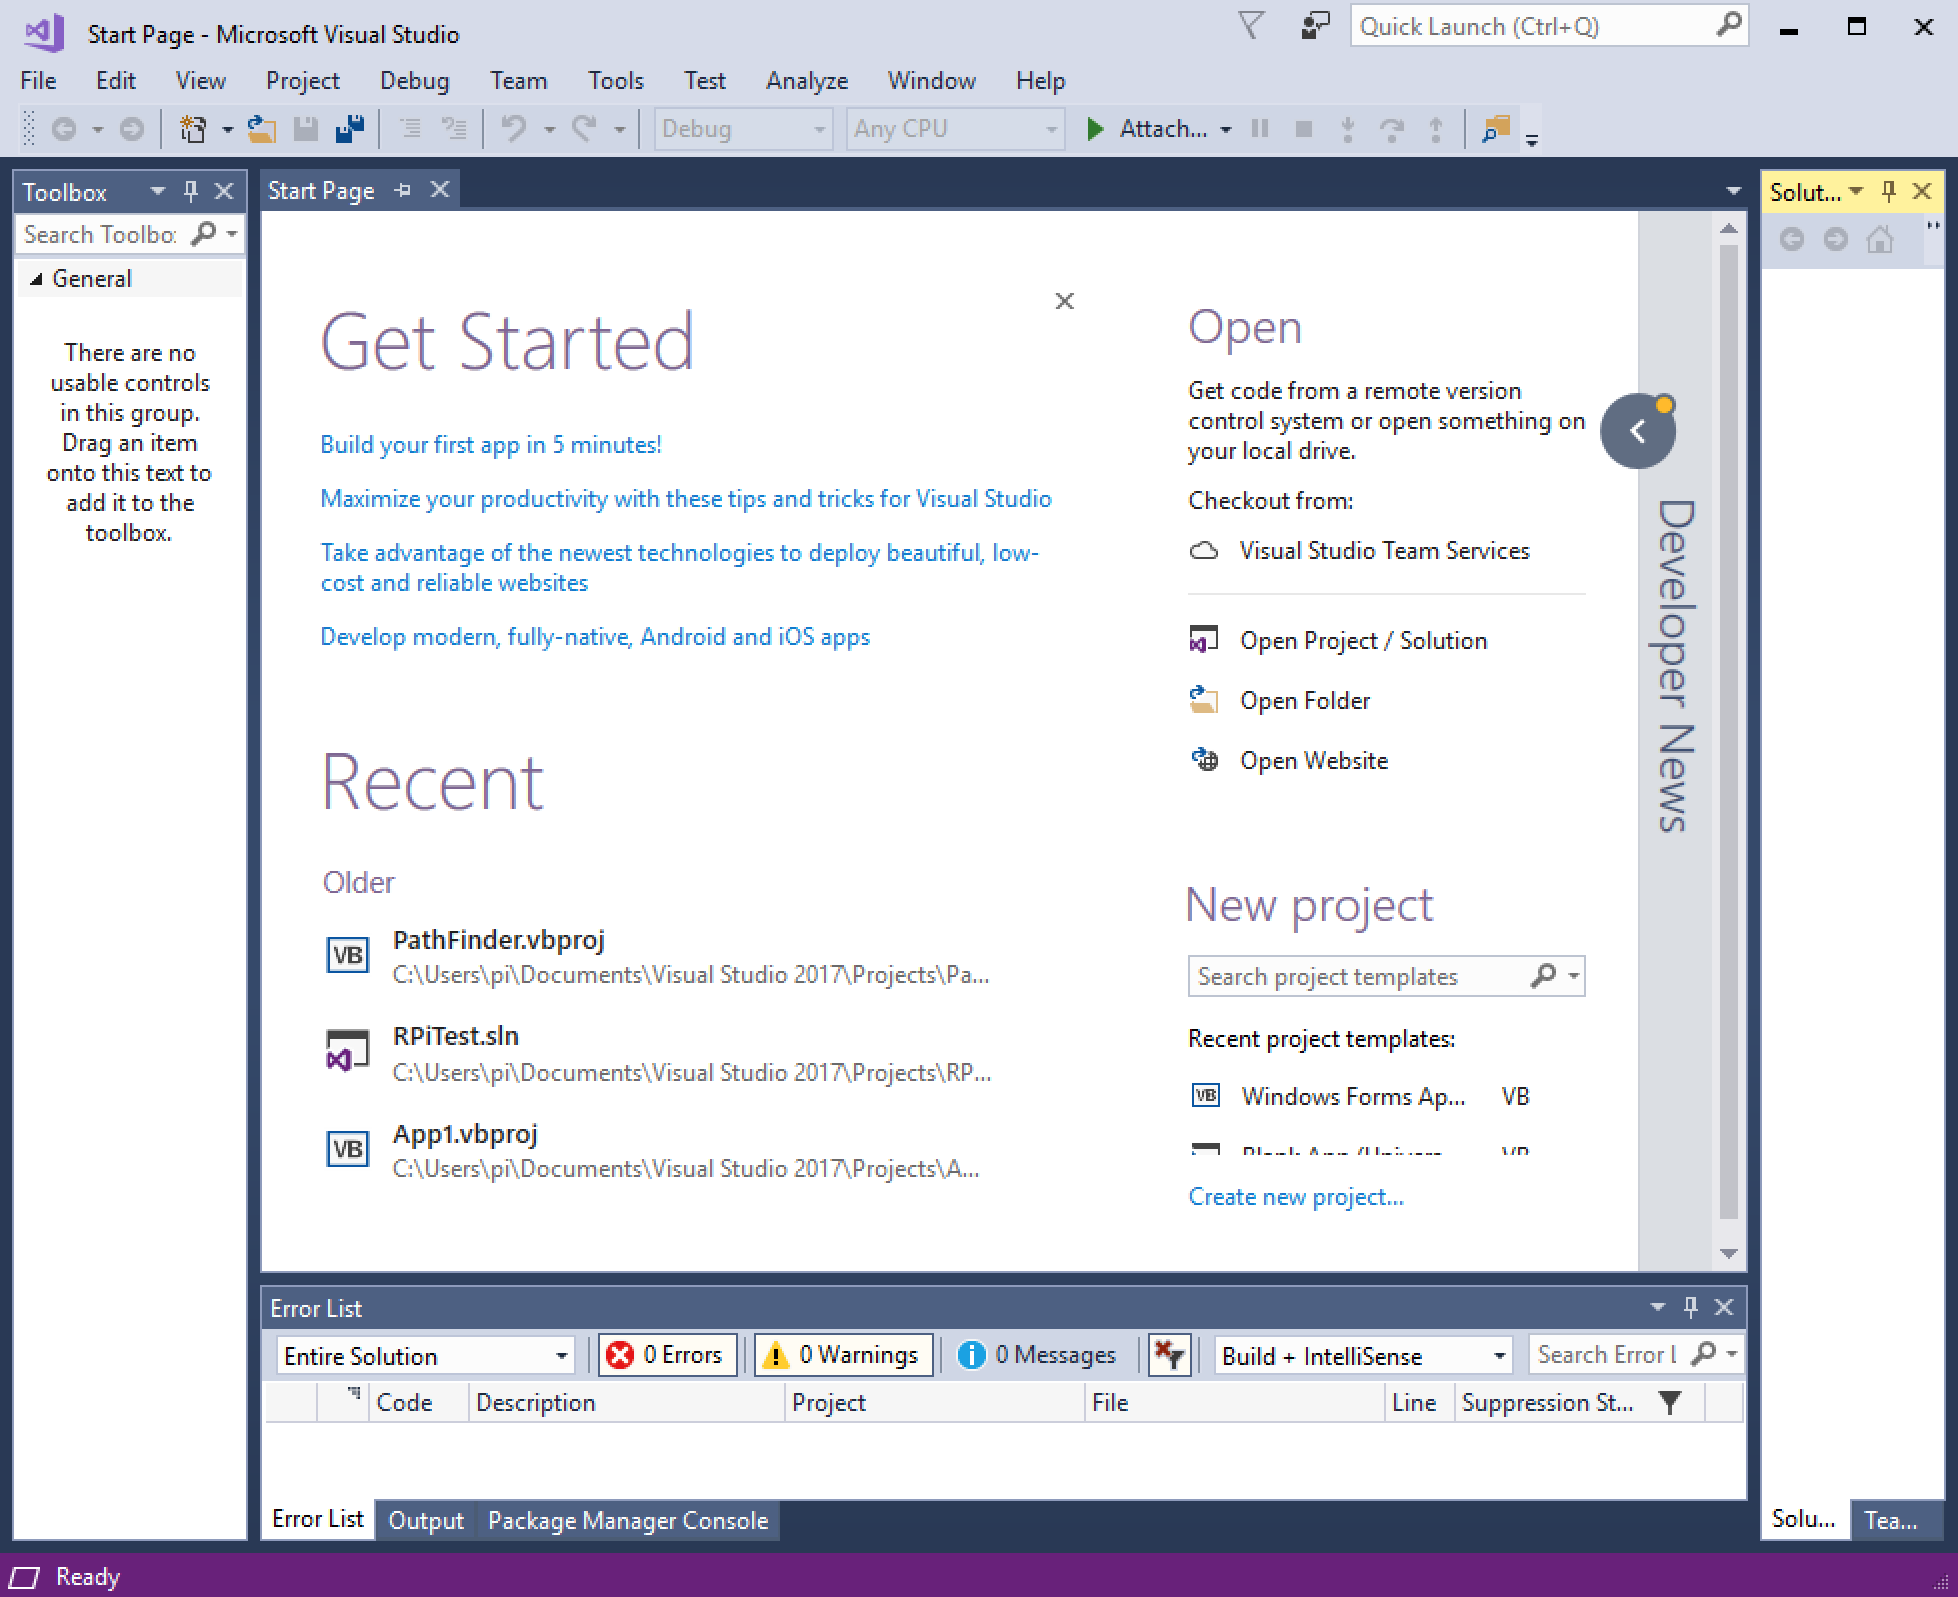
\includegraphics[width=\textwidth]{ide_startup}
			\caption{The Start Page.}
			\label{fig:ide_startup}
			\end{figure}

		\begin{figure}[ht]
			\centering
			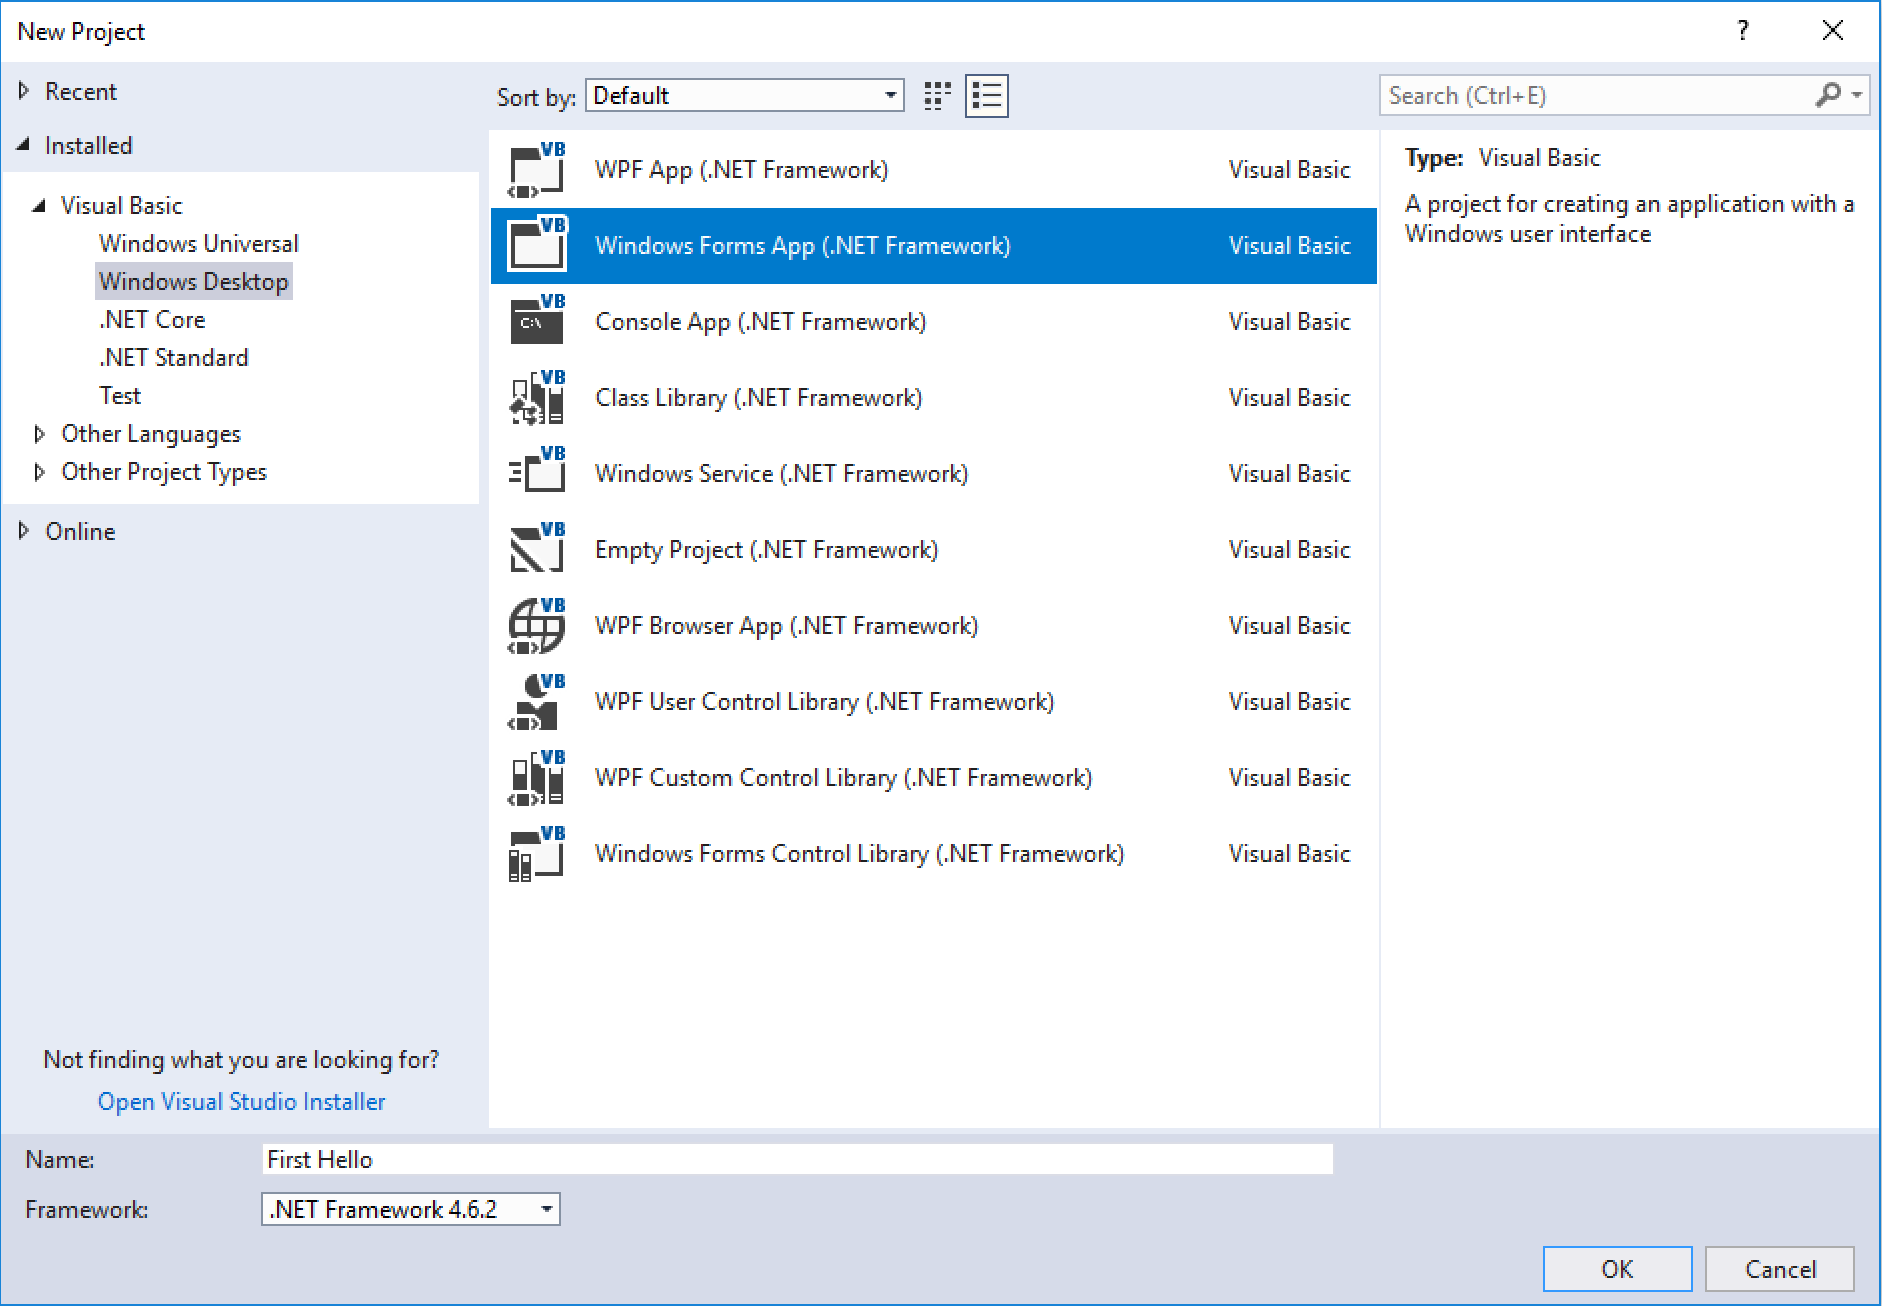
\includegraphics[width=\textwidth]{ide_new_project}
			\caption{The \ui{New Project} window.}
			\label{fig:ide_new_project}
		\end{figure}

		\begin{figure}[ht]
			\centering
			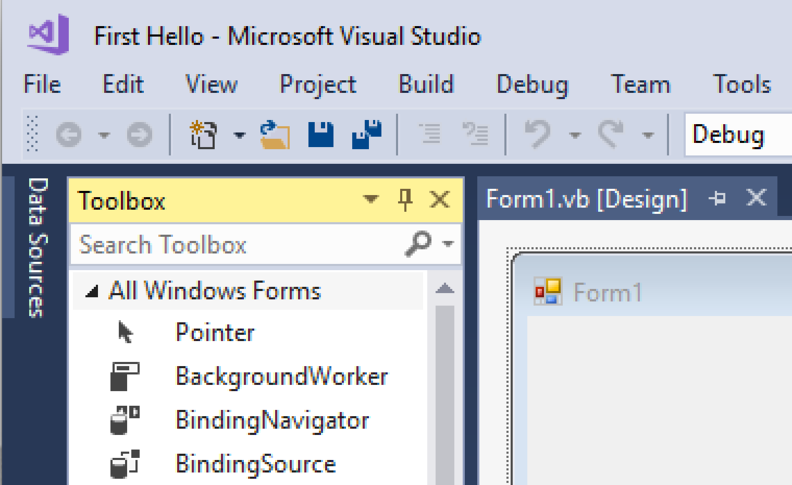
\includegraphics[width=8cm]{ide_toolbox}
			\caption{After pinning open the toolbox.}
			\label{fig:ide_toolbox}
		\end{figure}


		
		The above steps are typical for any project. Let us now do a specific task for this particular project.
Note the form and the toolbox in \Vref{fig:ide_ide_parts}. We are going to select a control from the toolbox and place it on the form. Here are the steps:
		\begin{itemize}
			\item	Locate the toolbox. Click on \ui{Label}.
			\item	Move the mouse to the form. Hold down the left button, and drag the mouse to create a label as in \Vref{fig:ide_form1}.
			\item	We will now set some properties of the label: right-click on the label and select \ui{Properties}. Move to the Properties list at the bottom right of the screen, as shown in \Vref{fig:ide_properties}.
			\item	Scroll down to the \keyword{Text} property, and replace the existing \keyword{Label1} with \keyword{Hello World}.
			\item	Now, we run the program by clicking the arrow at the top of the IDE (\Vref{fig:ide_start_debug}).
		\end{itemize}
		A new window appears, as in \Vref{fig:ide_running}. This is the program that you have created. It merely displays some text, but it is a proper window in the sense that you can move it, resize it and shut it down by clicking the \ui{x} at the top right corner. Experiment with the window, then close it.

		To save your program for future use:
		\begin{itemize}
			\item	Go to the \ui{File} menu, selecting the \ui{Save All} option. (We use a shorthand for such actions, writing it as \ui{File | Save All}.)
			\item	The \ui{Save Project} window appears, as in \Vref{fig:ide_save_project}. Ensure that \ui{Create directory for solution} is checked. Leave its other settings unaltered, and click \ui{Save}. When you do a save again, the same settings will be used automatically, and the \ui{Save Project} window will not appear.
		\end{itemize}
		You can now use \ui{File | Exit} to leave the IDE.

		When you return to VB later, your project name will appear on the start page, and can be opened with a single click. The work we did on setting up the project does not need to be repeated.

		\begin{figure}[ht]
			\centering
			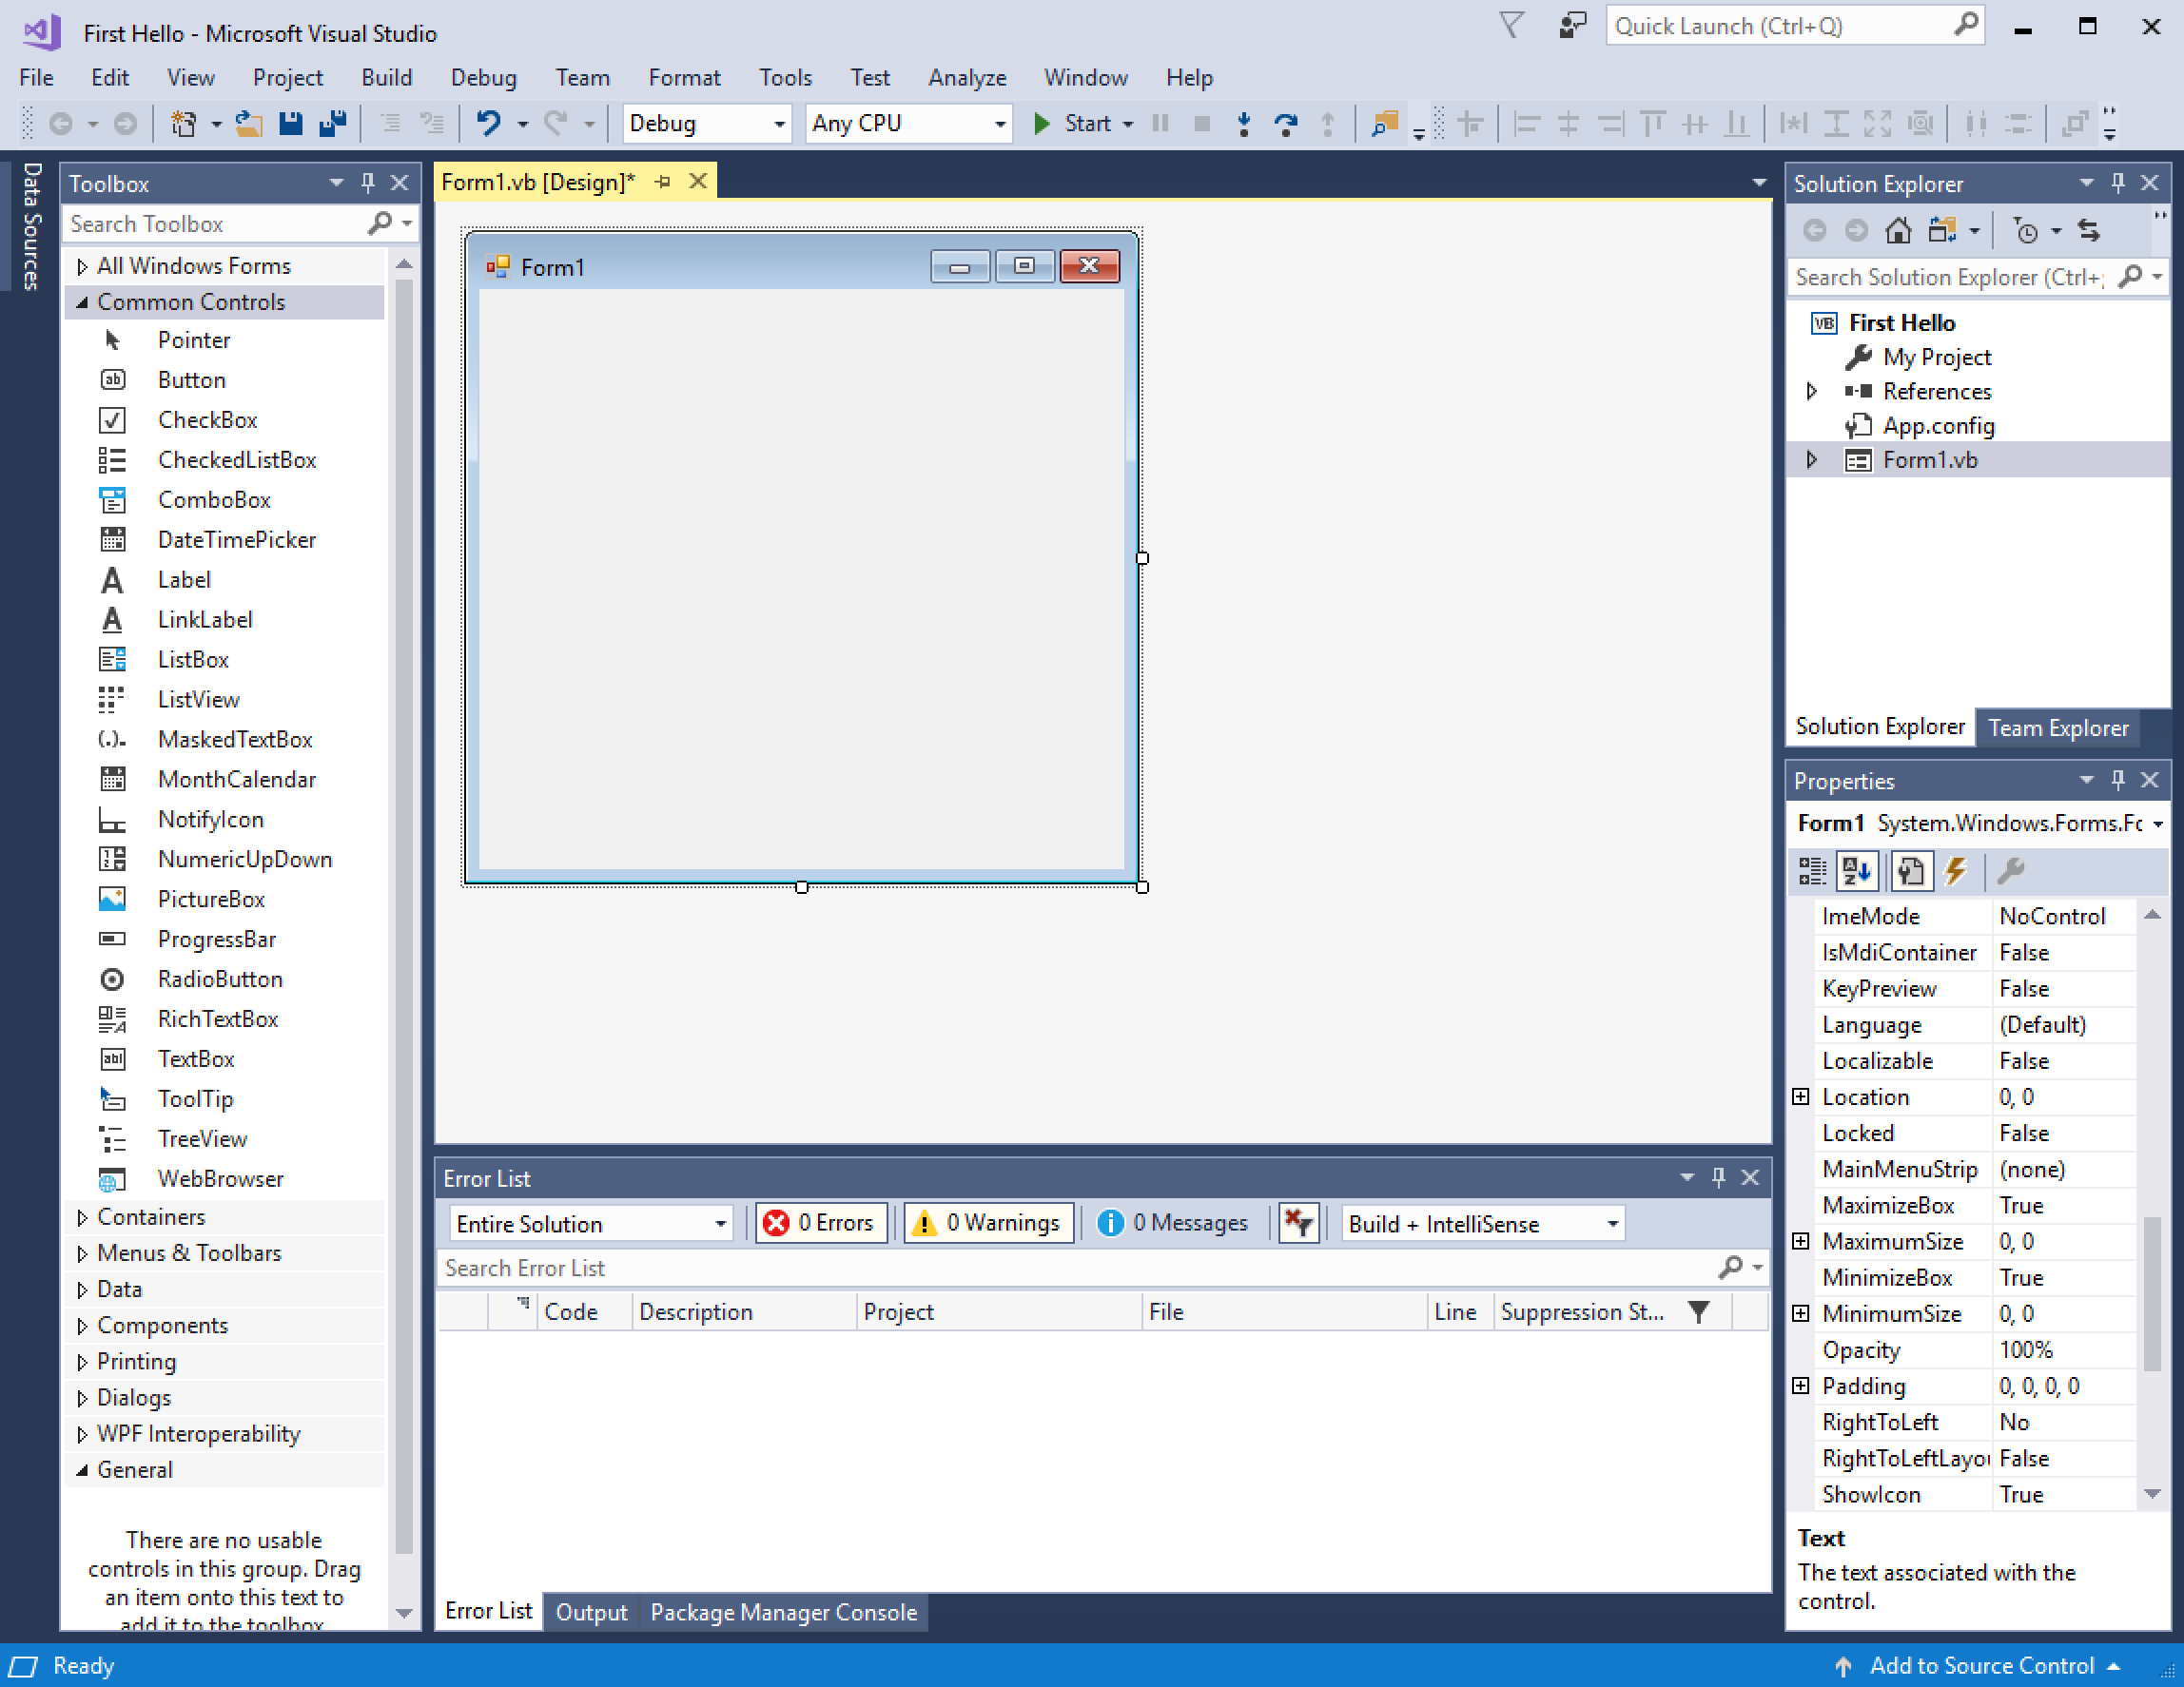
\includegraphics[width=\textwidth]{ide_ide_parts}
			\caption{The IDE at design-time.}
			\label{fig:ide_ide_parts}
		\end{figure}

		\begin{figure}[ht]
			\centering
			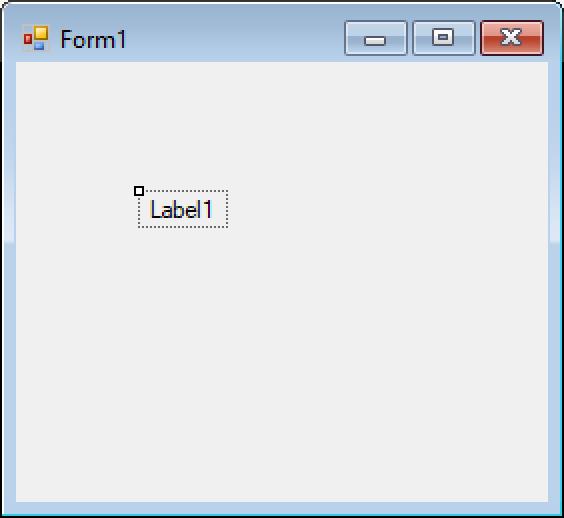
\includegraphics[width=7cm]{ide_form1}
			\caption{Form with label added.}
			\label{fig:ide_form1}
		\end{figure}

		\begin{figure}[ht]
			\centering
			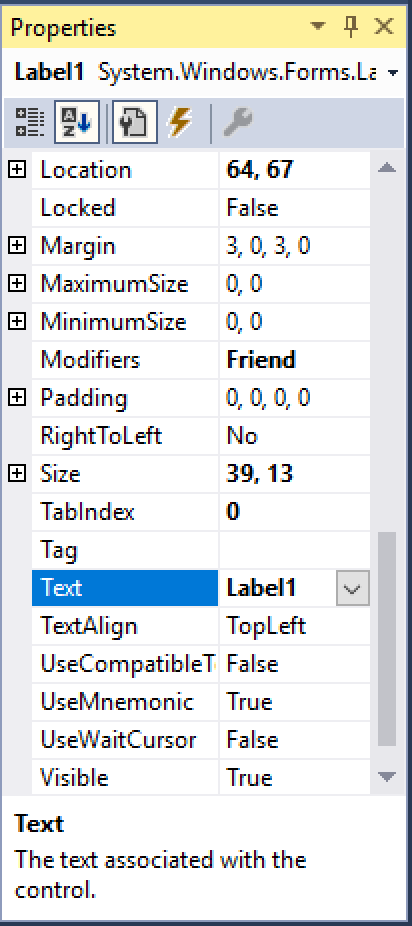
\includegraphics[width=3cm]{ide_properties}
			\caption{Properties of the label}
			\label{fig:ide_properties}
		\end{figure}
		\begin{figure}[ht]
			\centering
			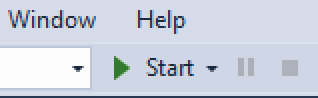
\includegraphics[width=3cm]{ide_start_debug}
			\caption{Click the arrow/ play button to run the program.}
			\label{fig:ide_start_debug}
		\end{figure}

		\begin{figure}[ht]
			\centering
			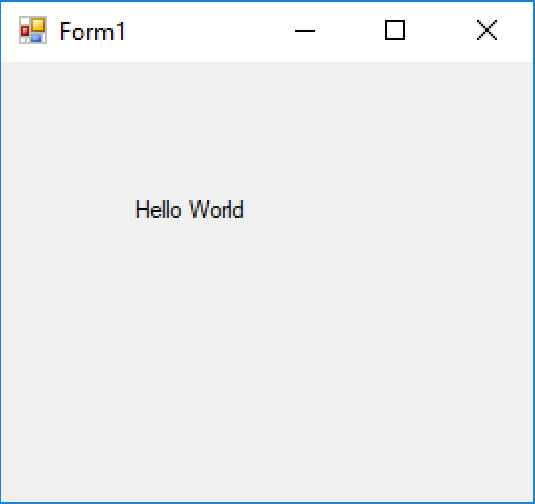
\includegraphics[width=7cm]{ide_running}
			\caption{Screenshot of running the First Hello program.}
			\label{fig:ide_running}
		\end{figure}

		\begin{figure}[ht]
			\centering
			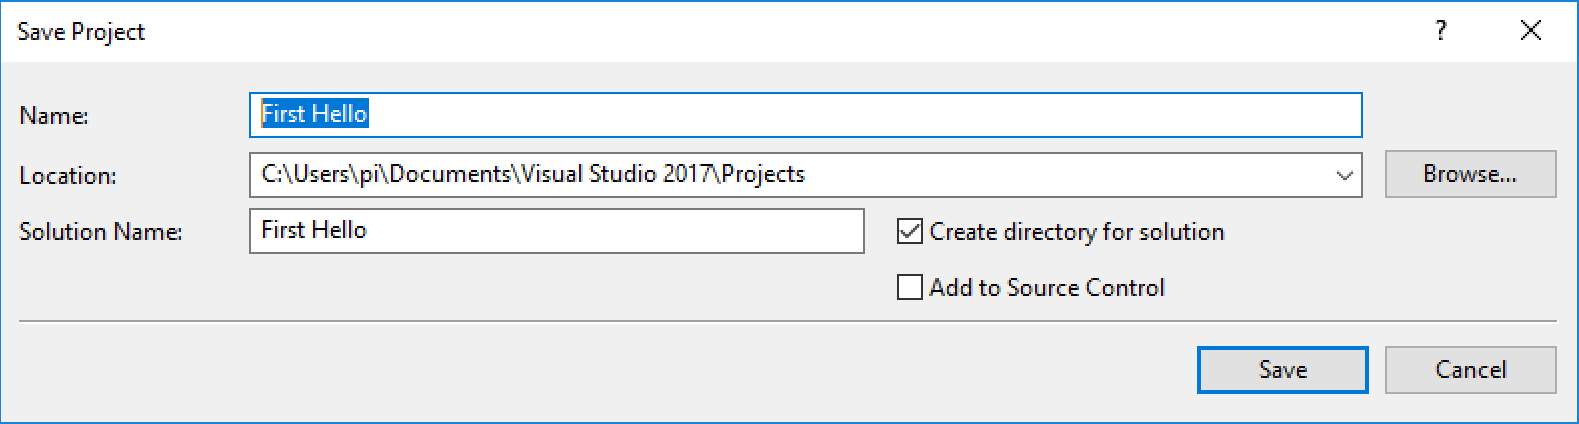
\includegraphics[width=12cm]{ide_save_project}
			\caption{The \ui{Save Project} window, with \ui{Create directory} checked.}
			\label{fig:ide_save_project}
		\end{figure}


	\section{Controls at design-time}
		In our First Hello program, we placed a label on a form and altered the text that it displayed. The main point of the exercise was to go through the steps involved in creating a project. Now we will fill in some of the principles of controls and properties.


		What \emph{is} a control? A control is a ‘gadget’ that appears on the screen, to display 
information, to allow user interaction, or both of these. The VB IDE itself uses many controls. For example, you have made use of the drop-down menus to save projects, and the \ui{OK} button to confirm actions. For Windows applications, the toolbox contains around 70 controls, and part of the programming task involves choosing appropriate controls, positioning them on a form, and setting their properties. This phase of using a control is termed \emph{design-time} to distinguish it from \emph{run-time}, when the program runs (executes) and the user interacts with the controls. We create a \emph{graphical user interface} (GUI) for the user. Let us examine how controls can be manipulated at design-time.
		\begin{itemize}
			\item	A control can be selected from the toolbox, and positioned on a form. The initial position is not crucial; it is easily changed.
			\item	We can move the control. Hold the mouse within a control. A four-headed arrow will appear, as in \Vref{fig:ide_control_move}. The control can now be dragged with the mouse. Temporary lines appear, to help you align several controls.
			\item	We can resize the control. Clicking on a control shows a number of small boxes (handles) on the edge of the control. Hold the mouse over one of them. A two-headed arrow appears, as in\Vref{fig:ide_control_resize}. Drag the edge or corner to resize the rectangle.
		\end{itemize}
		In fact, the approach to resizing depends on the particular control. For example, the label control has an \ui{AutoSize} property, which we set to \ui{False} in \Vref{fig:ide_control_resize}. If we left \ui{AutoSize} set to \ui{True}, the width of the label is determined by the width of the text it has to display, and its height is determined by the font size of the text. Some other controls allow the width to be dragged, but not the height. (We set the height via fonts.) Some controls – such as buttons – allow resizing in all directions. In general, resizing is intuitive, so explore. However, because labels are so common, don’t forget about their \ui{AutoSize} property.
	
		\begin{figure}[ht]
			\centering
			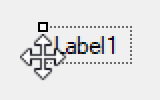
\includegraphics[width=3cm]{ide_control_move}
			\caption{Moving a control.}
			\label{fig:ide_control_move}
		\end{figure}

		\begin{figure}[ht]
			\centering
			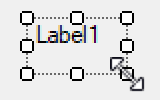
\includegraphics[width=3cm]{ide_control_resize}
			\caption{Resizing a control.}
			\label{fig:ide_control_resize}
		\end{figure}


		Now we will examine \emph{properties}. Here is an analogy: a television has properties, such as the colour of the case, the size of the screen, the current channel it is showing, its price, and its make.

		Each control has a set of properties, which we can adjust at design-time to meet our requirements. Later, we will see a property being changed at run-time.
		
		Once a control has been placed on a form, we can view its properties by right-clicking in it, and selecting \ui{Properties}. A properties window for the selected control will be shown. The left column contains the property names, and the right column contains the current value. To change a property, we modify the value in the right-hand column. For some properties, this might involve further selections, as in the settings of colours and fonts. Sometimes this involves opening up a further window where the range of values is large.
Another vital aspect of a control is its name. This is not in fact a property, but is shown in the properties list for convenience, as \ui(Name). The brackets indicate that it is not really a property.
When you place several labels on a form, the IDE chooses names in this fashion:
		\begin{lstlisting}
Label1 Label2 Label3 …
		\end{lstlisting}
		These are acceptable for now, but in future chapters we will suggest that you rename some controls, choosing meaningful names. A control is renamed by modifying the text to the right of \ui{(Name)} in the properties list.

		\begin{stqb}*
			\begin{STQ}
				\item	Place two labels on a form. Make the following changes to their properties. After each change, run the program, note the effect, and stop the program by clicking on X at the top-right corner.
					\begin{itemize}
						\item Move the labels;
						\item set the \ui{AutoSize} property of one of the labels to \ui{True};
						\item alter their \ui{Text} properties to display your name and age;
						\item alter their fonts;
						\item alter their back colour.
					\end{itemize}
				\item Select the form itself. Perform the following tasks, running the program after each change.
					\begin{itemize}
						\item Resize the form;
						\item alter its text property;
						\item alter its back colour property.
					\end{itemize}
			\end{STQ}
		\end{stqb}
		
	\section{Events and the Button control}
		The program we created earlier was unrepresentative, in the sense that it always displayed the same words, and no user interaction was possible. Now we will extend this program, so that some text is displayed when the user clicks a button. This is an example of using an event.

		Most events come from the user, and are generated when the user manipulates a control in some way at run-time. Each control has a number of events it can respond to, such as a single mouse-click, a double-click, or the mouse being held over the control. There are also other types of events that do not originate from a user – for example the notification that a web page has finished downloading.

		In the program that follows, we will detect an event (the click of a button), and then cause some text to be displayed in a label. Here is how we create the user interface:
		\begin{itemize}
			\item	create a new project named Hello Button;
			\item	place a label and a button on the form. The positioning is not crucial;
			\item set the \keyword{Text} property of the button to \keyword{Click Me};
			\item alter the \keyword{Text} property of the label so that it contains nothing.
		\end{itemize}
		The program is not yet complete, but run it. Note that you can click the button and it shifts slightly, to provide confirmation of the click; nothing else happens. Shut down the form.
		
		Now we will detect the click event. On the design form, double-click on the button. A new pane of information will open up, as in \Vref{fig:ide_tabs}. Note the tabs at the top, showing:
		\begin{lstlisting}
Form1.vb
Form1.vb [Design]
		\end{lstlisting}
		these can be clicked to switch panes. The \ui{Form1.vb} pane shows a VB program. We call this \emph{program text}, or VB \emph{code}. We are going to modify this code using the editor within the IDE.
Locate the section:
		\begin{lstlisting}
Private Sub Button1_Click (sender As … etc
End Sub
		\end{lstlisting}
		This section of code is termed a \emph{method}. The name of the method is \keyword{Button1\_Click}. When the user single-clicks on \keyword{Button1} at run-time, any instructions we place between the above two lines will be carried out, or ‘executed’. This is because the line ends with \keyword{Handles Button1\_Click}.
		
		In this particular program, we will use an instruction to place \keyword{Hello World} into the text of \keyword{Label1}. The instruction to do this is:
		\begin{lstlisting}
Label1.Text = "Hello World"
		\end{lstlisting}

		\begin{figure}[ht]
			\centering
			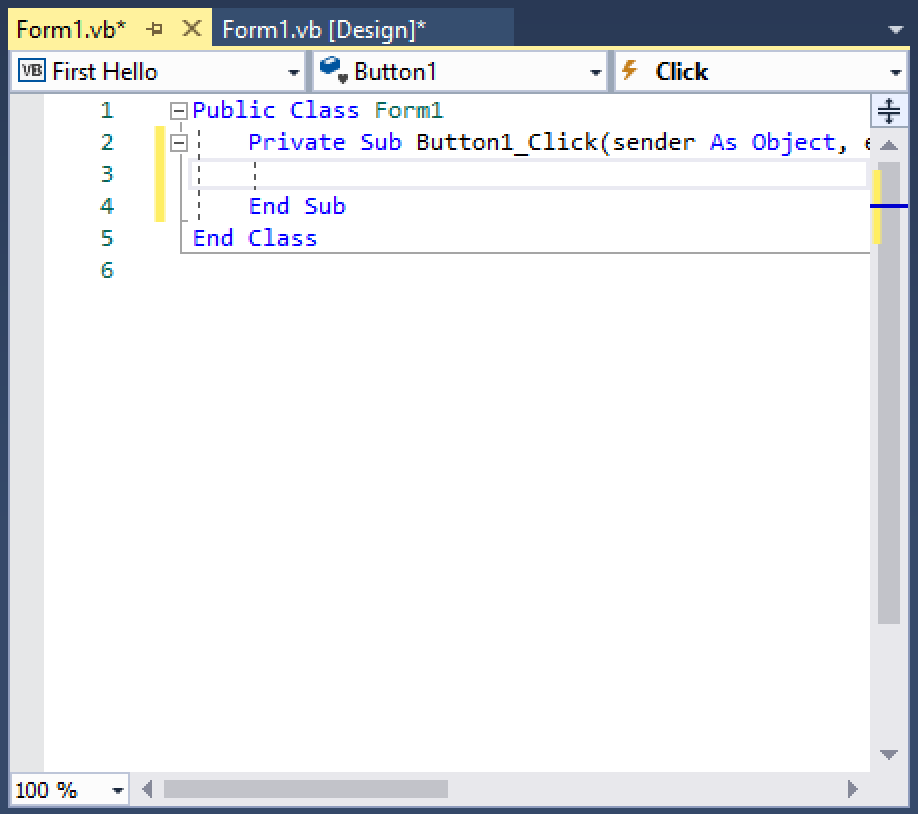
\includegraphics[width=10cm]{ide_tabs}
			\caption{VB code in the editor pane.}
			\label{fig:ide_tabs}
		\end{figure}

		
		Type it in exactly as shown, placing it between the \keyword{Private Sub} and the \keyword{End Sub} lines. Note carefully the last two characters of \keyword{Label1}. One of them is a lower-case \keyword{L}, and the other is the digit \keyword{1}. The exact meaning of lines such as this (which involves an ‘assignment statement’) will be explained in later chapters.

		The next step is to run the program. There are two possibilities:
		\begin{itemize}
			\item The program runs correctly. Click the button, and note that \keyword{Hello World} appears in the label.
			\item Alternatively, the program might not run, due to an error. In this case, VB displays a message as shown in \Vref{fig:ide_build_errors}. Check the box, and choose \ui{No}. The message will not appear again.
		\end{itemize}
		However, the error still needs fixing, so correct any errors in your typing, and run the program again. Errors are discussed in more detail below.

		The new features in this program are:
		\begin{itemize}
			\item It has responded to the click on a button. Placing code so that it is obeyed when an event occurs is termed ‘handling’ the event.
			\item It has altered the value of a control’s property at run-time. Previously, we only did this at design-time. This is a very important part of programming, because we often display results by placing them in a property of a control.
		\end{itemize}

		\begin{figure}[ht]
			\centering
			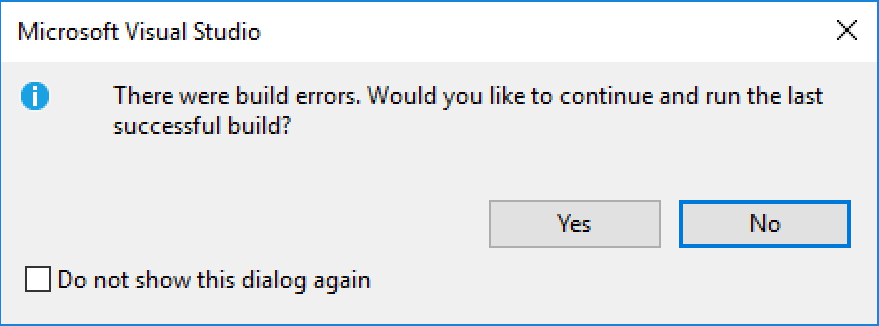
\includegraphics[width=10cm]{ide_build_errors}
			\caption{Error action. Check the box and click \ui{No}.}
			\label{fig:ide_build_errors}
		\end{figure}

		\begin{stqb}
			\begin{STQ}
				\item	Place a second label on the form. Make it show your name when the button is clicked.
			\end{STQ}
		\end{stqb}

	\section{Opening an existing project}
		To re-open a project that you created earlier, save and close any current project you are working on, and move to the Start Page. This displays your most recent projects. To open one, just click its name. If the project you want is not in the list, click the \ui{Open Project …} link, and browse to the appropriate folder. Inside the folder, there is a file of type \keyword{.sln} (solution). Select this, and open the project. To view the form, move to the Project Explorer at the top right side, and click on the form name to open it.
		
	\section{Documenting property settings}
		In this book, we need to provide you with the settings for controls. For a small number of properties, we can explain these in a few sentences of English, but for a larger number of properties, we will use a table. In general, we have a number of controls. Each control has a number of properties, and each property has a value. Note that 
there are a large number of properties for each control, but we only list the properties 
that you need to modify. The other properties keep their default setting. Here is an example:
		\begin{center}
			\begin{tabular}{lll}
				\toprule Control & Property & Setting\\ \midrule
				Label1 & Text & Hello World\\
				Label1 &BackColor & Red \\
				Button1 & Text & Click Me\\ \bottomrule
			\end{tabular}
		\end{center}
 		It represents:
			\begin{itemize}
				\item \keyword{Label1} with its text set to \keyword{Hello World}, and its background colour set to red;
				\item \keyword{Button1} with its text set to \keyword{Click Me}.
		\end{itemize}
		The spelling of property names should be followed carefully. This will be covered in more detail in later chapters, but for now, note that they start with a capital and do not contain spaces.
	\section{Program errors}
		It is common for mistakes to occur in programs, and the IDE will spot some of them for you. Here is an example of a mistake:
		\begin{lstlisting}
Label1.Tixt = "Hello World"
		\end{lstlisting}
		When you enter this line, the IDE will underline it. If you hold the mouse over the underlined part, an explanation of the error pops up. You should note that the explanation might be hard to understand (even for experts) or it might be that the error is in another part of the program. However, your first step is always to inspect the underlined area for spelling errors. As you learn more of the VB language, your ability to spot mistakes will improve.

		Once the underlined errors are corrected, we run the program. In fact, before the program runs, a program known as a compiler makes checks on it, and more errors might be detected. Only when all these compilation errors have been corrected will the program be allowed to run.

		Compilation errors are listed in the \ui{Error List} window, which opens below the code. Double-clicking on the error in the output window will take you to the point in the code where it can be corrected.

		Everyone who begins to write programs will encounter lots of compilation errors. Do not be dismayed. It is part of the learning process.

		Once the compilation errors have been fixed, the program will run. Then we might notice that it runs incorrectly – it has a ‘bug’. Such run-time errors are much harder to fix, and debugging is needed. We cover this in \Cref{ch:debugging}.

	\section{Editor facilities}
		The editor does more than just display what you type in. Here are some of its facilities.
		\begin{itemize}
			\item It provides standard clipboard cut, copy and paste, letting you copy code from other Windows programs.
			\item The writing of bigger programs involves more controls and more events. The drop-down lists at the top of the editor allow you to select a control, and a particular event for that control. The editor positions itself to the appropriate method.
			\item As you type in VB code, the editor will lay it out according to certain rules. For example, spaces will automatically be inserted around the = symbol.
			\item Some lines will be indented – shifted to the right – by the insertion of extra spaces. Normally, this is in steps of four spaces. As you will see in later chapters, VB code consists of sections within sections, and indentation clarifies where a section begins and ends.
			\item Some of the letters you type will be converted to capitals, according to the conventions of the VB language.
			\item Each type of control has a different set of properties. If you type in a control name followed by a dot, as in:
				\begin{lstlisting}
Label1.
				\end{lstlisting}
				then wait, the editor will provide a list of the label’s properties.
			\item Sections of code that we are not working on can be collapsed down to one line of code. This is done by clicking the small – at the left of the editor. Click + to expand a section. You will see these symbols alongside such lines as:
				\begin{lstlisting}
Private Sub Button1_Click(… etc
				\end{lstlisting}
		\end{itemize}
		You don’t have to remember these features – they are there to help you.

		One area of layout that is not done for you is the breaking up of long lines. To ensure that the whole of a line is visible on the screen, you can choose a suitable place to break the line. Spaces can then be inserted at the left to provide a suitable indentation. Here is an example, using this line:
		\begin{lstlisting}
Private Sub Button1_Click(sender As System.Object	… etc
		\end{lstlisting}
		We can set this out as:
		\begin{lstlisting}
Private Sub Button1_Click( 
	sender As System.Object, 
	e As System.EventArgs) Handles Button1.Click
		\end{lstlisting}
		Often, the very long lines are created by the IDE and should not contain errors. Breaking them is not essential. However, when you progress in VB, some of the 
long lines will be your creation, and it is well worth breaking them so that the whole text can be seen at once. The readability of printed code (called a listing) is also improved.

	\begin{stqb}
			\begin{STQ}
				\item	Place a label and a button on a form, then do the following:
					\begin{enumAlph}
						\item double-click on the button at design-time, and insert the line:
							\begin{lstlisting}
Label1.Tixt = "Doug"
							\end{lstlisting}
							Note the underlining, and the error message.
						\item Run the program. Note the error in the Error List, then double-click on it. Fix the error.
						\item Remove the spaces at the left of the line, and around the =. Click elsewhere in the code, and note the effect.
						\item Alter \keyword{Text} to \keyword{text}. Note the effect.
					\end{enumAlph}
			\end{STQ}
		\end{stqb}

	\section{The message box}
		Earlier, we used the label control to display text on the screen. We can also use a message box. This does not occur in the toolbox, because it occupies no permanent space on a form. Instead, it pops up when required. Here is some code which displays \keyword{Hello World} in a message box, when a button is clicked:
			\begin{lstlisting}
Private Sub Button1_Click(
	sender As System.Object,
	 As System.EventArgs) Handles Button1.Click
	MessageBox.Show("Hello World")
End Sub
			\end{lstlisting}

		Figure 2.14 shows what happens when we run the program and click the button. The message box appears, and we must click the \ui{OK} button to make it go away. This feature means that message boxes are used for vital messages that the user cannot ignore.

		To use a message box, key in a line just like the above, putting your own message inside the double quotes. At this point we will not explain the purpose of the Show, or why the brackets are needed. This comes later, when we study methods in more detail.
	\begin{stqb}
			\begin{STQ}
			\item	Write a program which has two buttons on a form. Clicking one button shows a message box containing \keyword{Hello World}. Clicking the other button shows a message box containing \keyword{Goodbye Cruel World}.
			\end{STQ}
		\end{stqb}

		
	\section{Help}
		The help system works from two possible sources: locally from your own computer, or from the Internet. The Internet one is updated frequently, and is the simplest to enter. To use this, set up your help system:
		\begin{enumerate}
			\item	Choose \ui{Help | Manage Help Settings}.
			\item	Click \ui{Choose online or local help}.
			\item	On the following screen, choose the \ui{online} option.
		\end{enumerate}
		To get help, click \ui{Help | View Help}. A web browser will run, opening Microsoft’s help site. You can enter items in the text box provided, and a list of found pages is displayed.

		The help results are not always geared to beginners, so alternatively you could try a popular search engine, entering such phrases as ‘Visual Basic Button example’. Ensure that you do not study pages concerned with Visual Basic version 6.

	\section{Programming principles}
		\begin{itemize}
			\item Controls can be positioned on a form at design-time.
			\item The properties of controls can be set at design-time.
			\item Programs can change properties at run-time.
			\item When an event (such as a button-click) happens, the VB system uses the matching method. We place code within the method to handle the event.
		\end{itemize}

	\section{Programming pitfalls}
		\begin{itemize}
			\item Forgetting to terminate your running program before trying to modify the form or code.
		\end{itemize}

	\section{Grammar spot}
	\begin{itemize}
		\item In VB code, we refer to the property of a control by using the control’s name, followed by a dot, followed by the property, as in:
			\begin{lstlisting}
Label1.Text
			\end{lstlisting}
		\item A section of code between:
			\begin{lstlisting}
Private Sub ...
End Sub
			\end{lstlisting}
			is termed a method.
		\item A message box is not placed on a form. Instead, we cause one to be displayed by using:
			\begin{lstlisting}
MessageBox.Show("Some text you choose")
			\end{lstlisting}
		\end{itemize}

	\section{New language elements}
		An introduction to properties, methods, events.

	\section{New IDE facilities}
		\begin{itemize}
			\item A program is contained in a project.
			\item The IDE creates a folder to contain the files needed for a project.
			\item The setting of the project options \ui{Strict} and \ui{Explicit}.
			\item We can move and resize the controls on a form.
			\item The toolbox contains a range of controls.
			\item Right-clicking on a control allows us to select its properties.
			\item Double-clicking on a control at design-time will create event-handling methods.
		\end{itemize}

	\section{Summary}
		Part of the programming task involves placing controls on a form and setting their initial properties. The VB IDE makes this task straightforward, but you need to practice with the IDE, as well as reading about it.

	\section{Exercises}
		\begin{enumChapter}
		\item Create a new project named Demo, and place three buttons on the form. Set their text to 1, 2, 3 respectively. Create three labels, and set their text to \keyword{A}, \keyword{B} and \keyword{C}. 
				Now place suitable code in the appropriate button methods so that:
				\begin{enumAlph}
				\item clicking Button1 sets the text of all the labels to \keyword{Yes};
				\item clicking Button2 sets the text of all the buttons to \keyword{No};
				\item clicking Button3 sets the text values back to \keyword{A, B, C}.
				\end{enumAlph}
			\item	This involves the use of the Visible property of a control, which can be set to \keyword{True} or \keyword{False}. For example, the following code makes \keyword{Label1} invisible:
				\begin{lstlisting}
Label1.Visible = False
				\end{lstlisting}
				Write a program with two buttons and one label. Clicking one button makes the label invisible, and clicking the other button makes it visible again.
			\item	This program involves the use of the \keyword{Image} property of the label, which makes the label display an image. Setting this property involves browsing for an image file. Choose any image you encounter: there are many sample images on most computers, and their file name often ends in \keyword{.jpg} or \keyword{.bmp}. Write a program with two buttons, and an image on a label. Clicking one button makes the image disappear. Clicking the other button makes it reappear.
			\item	Write a program which firstly displays your name in a message box, and then your age in a message box, when a button is clicked.
			\item	This involves the creation of a simple text editor. Place a text box on the form, and resize it so that it fills most of the form. Set its \keyword{Multiline} property to \keyword{True}, and its \keyword{ScrollBars} property to \keyword{Both}. Run the program. Type some text into the text box. Note that a right-click on the mouse allows cut and paste. Run a word-processor, and paste text to and from your editor.
			\item	This involves using the \keyword{MouseHover} event, which happens when the user holds the mouse over a control for a few seconds. To create a method that handles this event, place a button on the form, and, at the top of the text editor panel, select \keyword{Button1} and \keyword{MouseHover}. The method to handle the event is created. Write a program which displays a message box containing \keyword{Over Button} when the mouse is held over the button.
		\end{enumChapter}

		\begin{stab}
			\begin{enumChapter}
				\item	This question involves exploration; manipulating properties is a hands-on task. You will learn how to select controls and manipulate each one individually.
				\item	Note that the Text property affects the words that are shown in the title of the form.
				\item	At design-time, we clear the Text property of the label (which VB will have named as \keyword{Label2}). Then we add the following line:
					\begin{lstlisting}
Label2.Text = "Mike"
					\end{lstlisting}
				Place this line immediately below the line which displayed \keyword{Hello World}. Run the program.
				\item	
					\begin{enumAlph}
						\item Hold the mouse over the underlined part to see the pop-up error.
						\item The cursor will be positioned at the incorrect line. Change \keyword{Tixt} to \keyword{Text}.
						\item The IDE puts the spaces back.
						\item The IDE replaces the \keyword{t} with \keyword{T}.
					\end{enumAlph}
				\item	The following code is added to our message box example:
					\begin{lstlisting}
Private Sub Button2_Click( 
	sender As System.Object,
	e As System.EventArgs) Handles Button2.Click
	MessageBox.Show("Goodbye Cruel World")
End Sub
					\end{lstlisting}

			\end{enumChapter}
		\end{stab}
